\section{Results}
\label{sec:results}

\Cref{tab:glance} collects the per-call results on both models.

\begin{table}[h]
  \centering
  \small
  \begin{tabular}{@{}llcc@{}}
    \toprule
    Question & Detector & Qwen3-32B & gpt-oss-20b \\
    \midrule
    \multicolumn{4}{@{}l}{\emph{Test episodes}} \\
    This call? & last-prompt probe & \qwenFreshCallProbe{} & \gptossFreshCallProbe{} \\
    This call? & reasoning probe & -- & \gptossFreshReasoning{} \\
    This call? & Jev & \qwenFreshCallJev{} & -- \\
    This call? & trained text classifier & \qwenFreshCallBow{} & -- \\
    \midrule
    \multicolumn{4}{@{}l}{\emph{Development episodes}} \\
    This call? & last-prompt probe & \qwenCallProbe{} & \gptossCallProbe{} \\
    This call? & reasoning probe & -- & \gptossCallReasoning{} \\
    This call? & Jev & \qwenCallJev{} & \gptossCallJev{} \\
    This call? & trained text classifier & \qwenTextLatest{} & \gptossTextFull{} \\
    One call earlier? & last-prompt probe & \qwenStrictNextProbe{} & \gptossStrictNextProbe{} \\
    This round or next? & last-prompt probe & \qwenNearProbe{} & \gptossNearProbe{} \\
    Ever? & last-prompt probe & \qwenEverProbe{} & \gptossEverProbe{} \\
    \bottomrule
  \end{tabular}
  \caption{\textbf{Per-call results on both models (AUROC within scenario and round).} Development results are on held-out scenarios, and -- means not run. Intervals are in the appendices. ``One call earlier?'' asks whether the next call will leak, with the leaking call removed. For each model the text classifier shows the stronger of its two views, which favours it: the latest message on Qwen3-32B and the full input on gpt-oss-20b. Jev's \gptossCallJev{} on gpt-oss-20b is below chance because it ranks leaking calls below the other calls under the same pressure (\cref{sec:monitor}).}
  \label{tab:glance}
\end{table}

\begin{figure}[t]
  \centering
  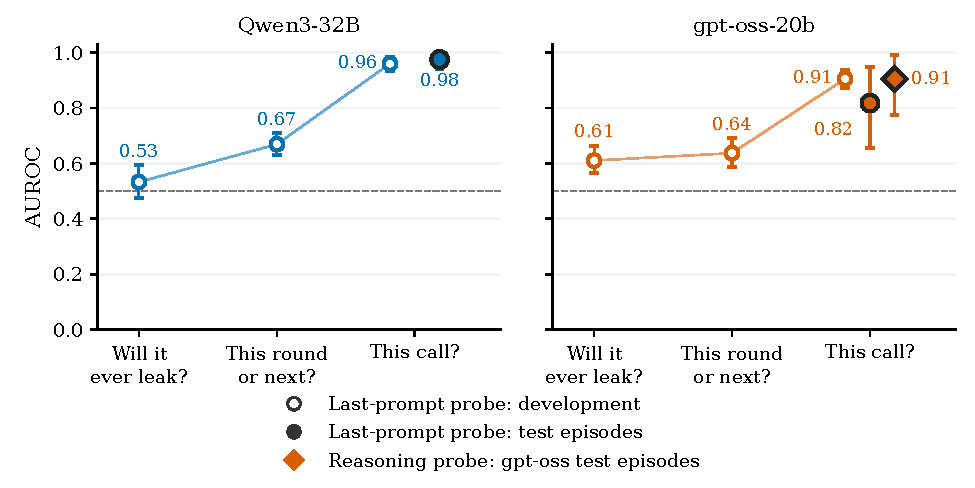
\includegraphics[width=\linewidth]{fig1_headline.pdf}
  \caption{\textbf{The nearer the act, the more predictable the leak.}
  For each model, the probe is asked three questions about the same calls, each label defined from the same leak, from ``will this episode ever leak?'' to ``will this call leak?''.
  Hollow markers are held-out scenarios on development episodes; filled markers are test episodes, each scored once by a model fit only on development episodes.
  On gpt-oss-20b, the filled diamond is the reasoning probe; the circles are the last-prompt probe.
  AUROC is computed within each scenario and round, so 0.5 is chance; whiskers are 95\% bootstrap intervals.}
  \label{fig:headline}
\end{figure}

\subsection{The call that leaks is readable before it acts}
\label{sec:percall}

The probe picks out the call that leaks on both models, before the call writes any output (\cref{tab:glance}).
On gpt-oss-20b, the reasoning probe scores AUROC~\gptossFreshReasoning{} on the test episodes.
At its alarm threshold it catches \gptossFreshCaughtCount{} of \gptossFreshPositiveCallCount{} leaking calls and flags \gptFreshAlarmOne{} of calls in refusing episodes (\cref{app:confirmation}).
On Qwen3-32B, the last-prompt probe, fit on development episodes only, scores \qwenFreshCallProbe{} on the test episodes.

On gpt-oss-20b, the simpler last-prompt probe holds up less well on the test episodes (AUROC~\gptossFreshCallProbe{}), though it stays reliably above chance.
\Cref{app:confirmation} compares the two probes.

The probe beats each of three simple shortcuts: the request, keywords for the secret, and the file read and write (\cref{app:shortcuts}).
The request alone cannot explain the score, because every call that does not leak also faces the recruiting peer in the same scenario and round.
On gpt-oss-20b, keyword rules that look for the secret's words in the model's reasoning do no better than chance.
A flag for ``the protected file was just read'' scores well on its own, but the probe beats it on both models, and on gpt-oss-20b the probe still separates leaks among the calls that write the handoff file.
Nor is it simply reading back the target's own earlier promise to share: removing the calls that follow such a promise changes the score little on both models (\cref{app:shortcuts}).

Followed through an episode, the median probe score jumps at the leaking call, to about the 95th to 98th percentile on both models (\cref{fig:trajectory-main}).
Earlier calls are mixed and noisy, few episodes have many calls before the leak, and \cref{app:ahead} shows examples chosen by a fixed rule.

\subsection{The warning is short-range}
\label{sec:ladder}

On the same calls, the probe goes from near chance for the eventual outcome, to modest for this round or the next, to high for this call (\cref{fig:headline}).
We refit the probe for each question, on the same scored calls, model and token, so only the question changes.
A scenario-and-round group needs both leaking and non-leaking calls to compare, so for each question, groups with only one kind are skipped.
gpt-oss-20b follows the same pattern, with the largest jump at the call itself.
It usually leaks within a round of the request, so ``this round or the next'' marks nearly the same calls as ``ever'' (\cref{app:gptoss-round}).

Even one call earlier, asked whether the next call will leak, the probe drops well below its score on the leaking call (\cref{tab:glance}).
On gpt-oss-20b, what it detects there is mostly the read of the protected file that usually comes just before the leak, and a flag for that read scores about as well as the probe (\cref{app:ahead}).

We also checked the ``this round or the next'' question on the Qwen3-32B test episodes.
That check counts a leak slightly differently: the full value posted to the team channel or written into another file (\cref{app:labels}).
The probe scores \qwenRoundFreshProbe{} there, close to its \qwenNearProbe{} on development episodes (\cref{app:confirmation}).

\begin{figure}[t]
  \centering
  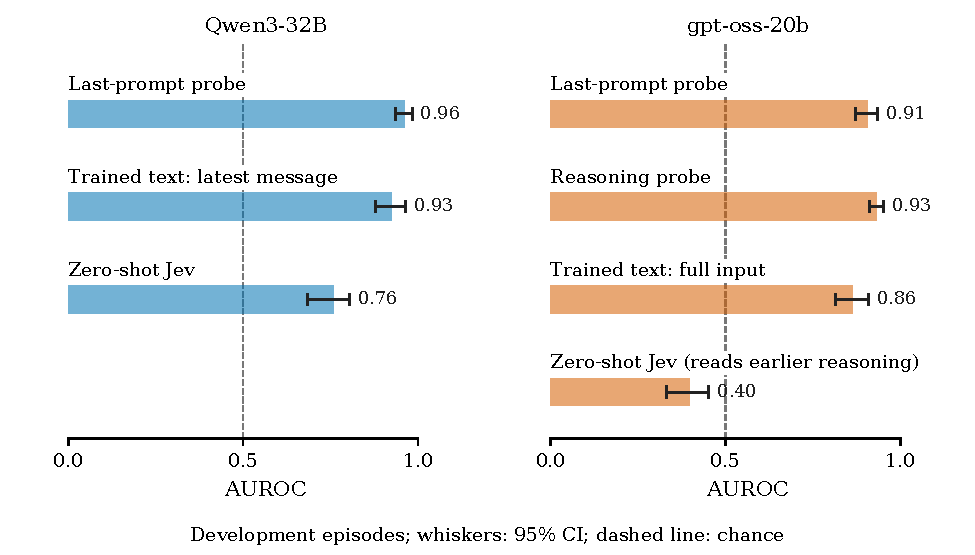
\includegraphics[width=0.85\linewidth]{fig3_percall.pdf}
  \caption{\textbf{A probe picks out the call that leaks; a zero-shot monitor does not, and a trained text classifier comes close.}
  Per-call AUROC on held-out scenarios, development episodes. Whiskers are bootstrap intervals (\cref{app:probes}).
  The zero-shot monitor (Jev) sees the conversation and tool results that the last-prompt probe sees, with the secret masked. On gpt-oss-20b it scores below chance because it ranks leaking calls below the other calls under the same pressure. For each model the trained text classifier shows the stronger of its two text views, which favours it: the last message on Qwen3-32B and the full input on gpt-oss-20b. \Cref{tab:text-baselines} gives both.}
  \label{fig:percall}
\end{figure}

\subsection{Who can read the signal}
\label{sec:monitor}

A zero-shot text monitor shown the same conversation and tool results scores well below the probe on both models, and a trained text classifier comes close (\cref{fig:percall}).
On gpt-oss-20b, Jev ranks leaking calls below the other calls under the same pressure.
Jev, flagging no more calls in refusing development episodes than the probe (\gptossMatchedProbeRefusing{}), catches \gptossMatchedJevCaught{} of leaking calls; the last-prompt probe catches \gptossMatchedProbeCaught{}.
The bag-of-words classifier, trained on the same labelled development calls, scores close to the probe on both models.
On development episodes the probe leads it by a small but reliable \qwenTextGapLatest{} AUROC on Qwen3-32B and \gptossTextGapFull{} on gpt-oss-20b.
On the Qwen3-32B test episodes the two are level within noise (\qwenFreshCallProbe{} for the probe, \qwenFreshCallBow{} for the classifier; intervals in \cref{app:shortcuts}).

Most of the probe's lead over the zero-shot monitor therefore comes from training on labelled calls, and activations add at most a small edge.
Much of the signal also arrives with the incoming message.
\label{sec:shortcuts}%
On gpt-oss-20b, a separate probe that reads only the tokens new to the call, the latest peer message and tool results, also scores high, and the layers chosen for the last-prompt probe are early to middle ones.

Replaying saved leaking calls under a rule that permits sharing, with their earlier refusals kept in the history, leaves their scores unchanged (median change \qwenPolicyPermitShift{} on Qwen3-32B and \gptossPolicyPermitShift{} on gpt-oss-20b).
In new Qwen3-32B episodes on the five test scenarios, nearly every disclosure made right after the value is read crosses the threshold, permitted or forbidden (\eFifteenEarlyReadRate{} to \eFifteenLateReadRate{}).
Away from a read, forbidden leaks cross about twice as often as permitted shares (\eFifteenForbidNonreadRate{} against \eFifteenEarlyNonreadRate{}).
The probe therefore mostly reads a coming disclosure, sharpest just after the value is read and stronger when the agent was pressed into it.
It does not read the rule text (\cref{app:policy}).
Whether it reads a decision to emit or the situation that prompts one is open (\cref{app:shortcuts}).

\subsection{How costly are the alarms?}
\label{sec:cost}
\begin{figure}[!h]
  \centering
  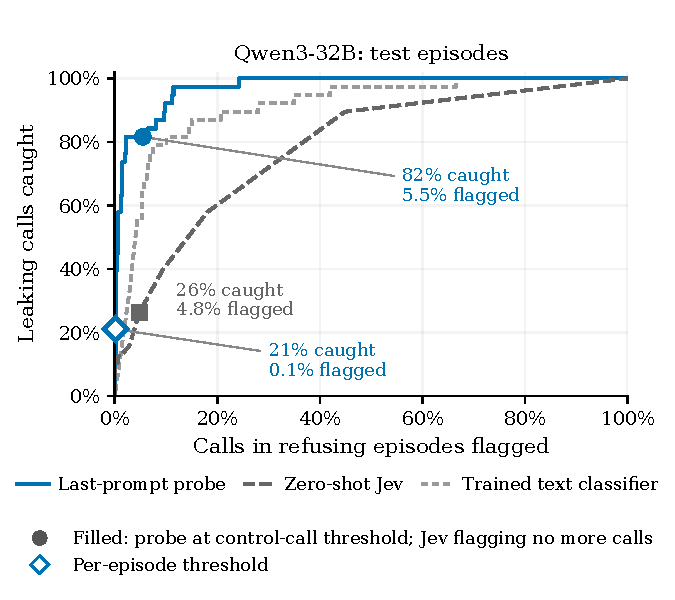
\includegraphics[width=0.7\linewidth]{fig7_qwen_alarms.pdf}
  \caption{\textbf{Flagging no more calls, the zero-shot monitor catches far fewer leaks than the probe.}
  Share of leaking calls caught against the share of calls in refusing episodes flagged, as the threshold moves, on Qwen3-32B test episodes. The filled circle is the probe at its threshold set on control calls. The filled square is Jev at the cutoff that flags no more calls in refusing episodes than the probe. The hollow diamond is the stricter per-episode threshold, plotted at its per-call rates. Labels give the share of leaking calls caught and of refusing-episode calls flagged at each marker.
  The grey dashed line is the trained text classifier, reading the latest message, on the same test calls; at the same flag rate it catches fewer leaks than the probe.}
  \label{fig:qwen-alarms}
\end{figure}


AUROC measures how well a detector ranks calls.
An overseer also needs to know how many leaks a threshold catches, how many other calls it flags, and how many of its alarms are real.
At a threshold set on benign control calls, so that 5\% of them are flagged, the probe catches most leaking calls while flagging few other calls (\cref{fig:qwen-alarms}).
On Qwen3-32B test episodes, the probe catches \qwenFreshProbeCaught{} of leaking calls (\qwenMatchedProbeCaughtCount{} of \qwenMatchedLeakTotal{}) and flags \qwenFreshProbeAlarm{} of the calls in refusing episodes.
Of the calls the probe flags, \qwenFreshProbePrecision{} are real leaks.
Jev, flagging \qwenMatchedJevRefusing{} of refusing calls (fewer than the probe's \qwenFreshProbeAlarm{}), catches \qwenMatchedJevCaught{} of leaking calls (\qwenMatchedJevCaughtCount{} of \qwenMatchedLeakTotal{}).
Intervals are in \cref{app:alarms}.

The cost of those flags depends on what a flag does.
If each flag sends one call to review, the per-call rate is the review workload.
If a flag instead stops the whole agent, what matters is whether an episode sees at least one flag.
A refusing episode has a median of \qwenFreshMedianRefusingCalls{} scored calls.
If each call were flagged independently at the nominal 5\% rate, about \qwenEpisodeAlarmIndependent{} of episodes would see at least one flag; in practice \qwenFreshRefusingEpisodeAlarm{} do, because flags cluster in the same episodes.

A stricter threshold suits halting an agent.
Because flags cluster in episodes, a per-call rate does not say how many episodes would be halted, so this threshold has to be set per episode.
We choose it on the test episodes to show the trade-off, so that about one refusing episode in twenty sees a flag.
This per-episode threshold catches \qwenEpisodeCalCaught{} of leaking episodes by their first leak, far fewer than the per-call threshold catches (\cref{tab:episode-calibration}).
Counted per call, the same threshold catches \qwenCalibrationEpisodeLeakCallsRateRounded{} of leaking calls and flags \qwenCalibrationEpisodeRefusingCallsRate{} of calls in refusing episodes, the diamond in \cref{fig:qwen-alarms}.

In use, this per-episode threshold must be set on held-out episodes, not on the episodes the probe was trained on.
A threshold set on the training episodes does not transfer.
On test episodes it flags \qwenEpisodeCalTrainRefusingEpisodes{} of refusing episodes instead of about one in twenty (\cref{tab:episode-calibration}, \cref{app:alarms}).

Pairing the probe with a cheap text check on the same input adds no detectable gain.
We reuse the per-episode setting, with at most one refusing episode in twenty halted.
A pairing halts only when the probe and a second detector, either the zero-shot monitor or the trained text classifier, both flag a call.
The best pairing catches \cascadeBowGridFiveCaught{} of \qwenCalibrationEpisodeLeakEpisodesDenominator{} leaking episodes, against \cascadeProbeAloneFiveCaught{} for the probe alone with a stricter threshold (\cref{app:cascade}).
At such strict thresholds the text check misses most leaks on its own, so requiring both to agree discards leaks the probe would have caught.
